% 	Name		:: 	sthlm Beamer Theme  HEAVILY based on the hsrmbeamer theme (Benjamin Weiss)
%	Author		:: 	Mark Hendry Olson (mark@hendryolson.com)
%	Created		::	2013-07-31
%	Updated		::	June 18, 2015 at 08:45
%	Version		:: 	1.0.2
%	Email		:: 	hendryolson@gmail.com
%	Website		:: 	http://v42.com
%
% 	License		:: 	This file may be distributed and/or modified under the
%                  	GNU Public License.
%
%	Description	::	This presentation is a demonstration of the sthlm beamer
%					theme, which is HEAVILY based on the HSRM beamer theme created by Benjamin Weiss
%					(benjamin.weiss@student.hs-rm.de), which can be found on GitHub
%					<https://github.com/hsrmbeamertheme/hsrmbeamertheme>.


%-=-=-=-=-=-=-=-=-=-=-=-=-=-=-=-=-=-=-=-=-=-=-=-=
%
%        LOADING DOCUMENT
%
%-=-=-=-=-=-=-=-=-=-=-=-=-=-=-=-=-=-=-=-=-=-=-=-=

\documentclass[newPxFont]{beamer}
\usetheme{sthlm}
%\usecolortheme{sthlmv42}

%-=-=-=-=-=-=-=-=-=-=-=-=-=-=-=-=-=-=-=-=-=-=-=-=
%        LOADING PACKAGES
%-=-=-=-=-=-=-=-=-=-=-=-=-=-=-=-=-=-=-=-=-=-=-=-=
\usepackage[utf8]{inputenc}
\usepackage[T1]{fontenc}

%\usepackage{chronology}
\usepackage{chronosys}
\usepackage{subfigure}

\newcommand{\tabitem}{%
  \usebeamertemplate{itemize item}\hspace*{\labelsep}}


%\renewcommand{\event}[3][e]{%
%  \pgfmathsetlength\xstop{(#2-\theyearstart)*\unit}%
%  \ifx #1e%
%    \draw[fill=black,draw=none,opacity=0.5]%
%      (\xstop, 0) circle (.2\unit)%
%      node[opacity=1,rotate=45,right=.2\unit] {#3};%
%  \else%
%    \pgfmathsetlength\xstart{(#1-\theyearstart)*\unit}%
%    \draw[fill=black,draw=none,opacity=0.5,rounded corners=.1\unit]%
%      (\xstart,-.1\unit) rectangle%
%      node[opacity=1,rotate=45,right=.2\unit] {#3} (\xstop,.1\unit);%
%  \fi}%

%-=-=-=-=-=-=-=-=-=-=-=-=-=-=-=-=-=-=-=-=-=-=-=-=
%        BEAMER OPTIONS
%-=-=-=-=-=-=-=-=-=-=-=-=-=-=-=-=-=-=-=-=-=-=-=-=

%\setbeameroption{show notes}

%-=-=-=-=-=-=-=-=-=-=-=-=-=-=-=-=-=-=-=-=-=-=-=-=
%
%	PRESENTATION INFORMATION
%
%-=-=-=-=-=-=-=-=-=-=-=-=-=-=-=-=-=-=-=-=-=-=-=-=

\title{Une approche par les Communs}
\subtitle{Ma vision}
%\date{\small{\jobname}}
%\date{\today}
\author{\texttt{E. Delay}\\
 une réflexion animée par \texttt{S. Aubert} et \texttt{A. Botta}}
\institute{CIRAD -- UMR SENS}

\hypersetup{
pdfauthor = {E. DELAY},
pdfsubject = {Attelier de Claret},
pdfkeywords = {Atelier finale de la CP1)},
pdfmoddate= {D:\pdfdate},
pdfcreator = {}
}

\begin{document}

%-=-=-=-=-=-=-=-=-=-=-=-=-=-=-=-=-=-=-=-=-=-=-=-=
%
%	TITLE PAGE
%
%-=-=-=-=-=-=-=-=-=-=-=-=-=-=-=-=-=-=-=-=-=-=-=-=


\maketitle

%\begin{frame}[plain]
%	\titlepage
%\end{frame}

%-=-=-=-=-=-=-=-=-=-=-=-=-=-=-=-=-=-=-=-=-=-=-=-=
%
%	TABLE OF CONTENTS: OVERVIEW
%
%-=-=-=-=-=-=-=-=-=-=-=-=-=-=-=-=-=-=-=-=-=-=-=-=
% \section*{Une boussole ?}
% \begin{frame}{Overview}
% % For longer presentations use hideallsubsections option
% \tableofcontents[hideallsubsections]
% \end{frame}

%-=-=-=-=-=-=-=-=-=-=-=-=-=-=-=-=-=-=-=-=-=-=-=-=
%	FRAME: INTRODUCTION
%-=-=-=-=-=-=-=-=-=-=-=-=-=-=-=-=-=-=-=-=-=-=-=-=

\section{Introduction :\\ L'approche par les Communs}


\begin{frame}[c]{L'urgence socio-environnementale}
  \vspace{-1cm}
  \begin{columns}[onlytextwidth,T]
    \column{\dimexpr\linewidth-30mm-5mm}

    l'anthropocène -- \textbf{événement frontière} (Haraway, 2016).
  
    Le capitalisme a suscité l'apparition de vivant profitant des différents bouleversements causés par ce qui a été appelé « progrès » pour se propager. (Stengler 2022)
    
    \textbf{Sentir l'effroi} -- apprendre l'art de l'attention, car rien n'y est plus garanti (Anna Tsing 2022)

    \begin{itemize}
      \item faits de violence et de guerre,
      \item appropriation des terres,
      \item artificialisation -- plantations,
      \item \textit{etc.}
    \end{itemize}

    \column{30mm}
    \vspace{2cm}
    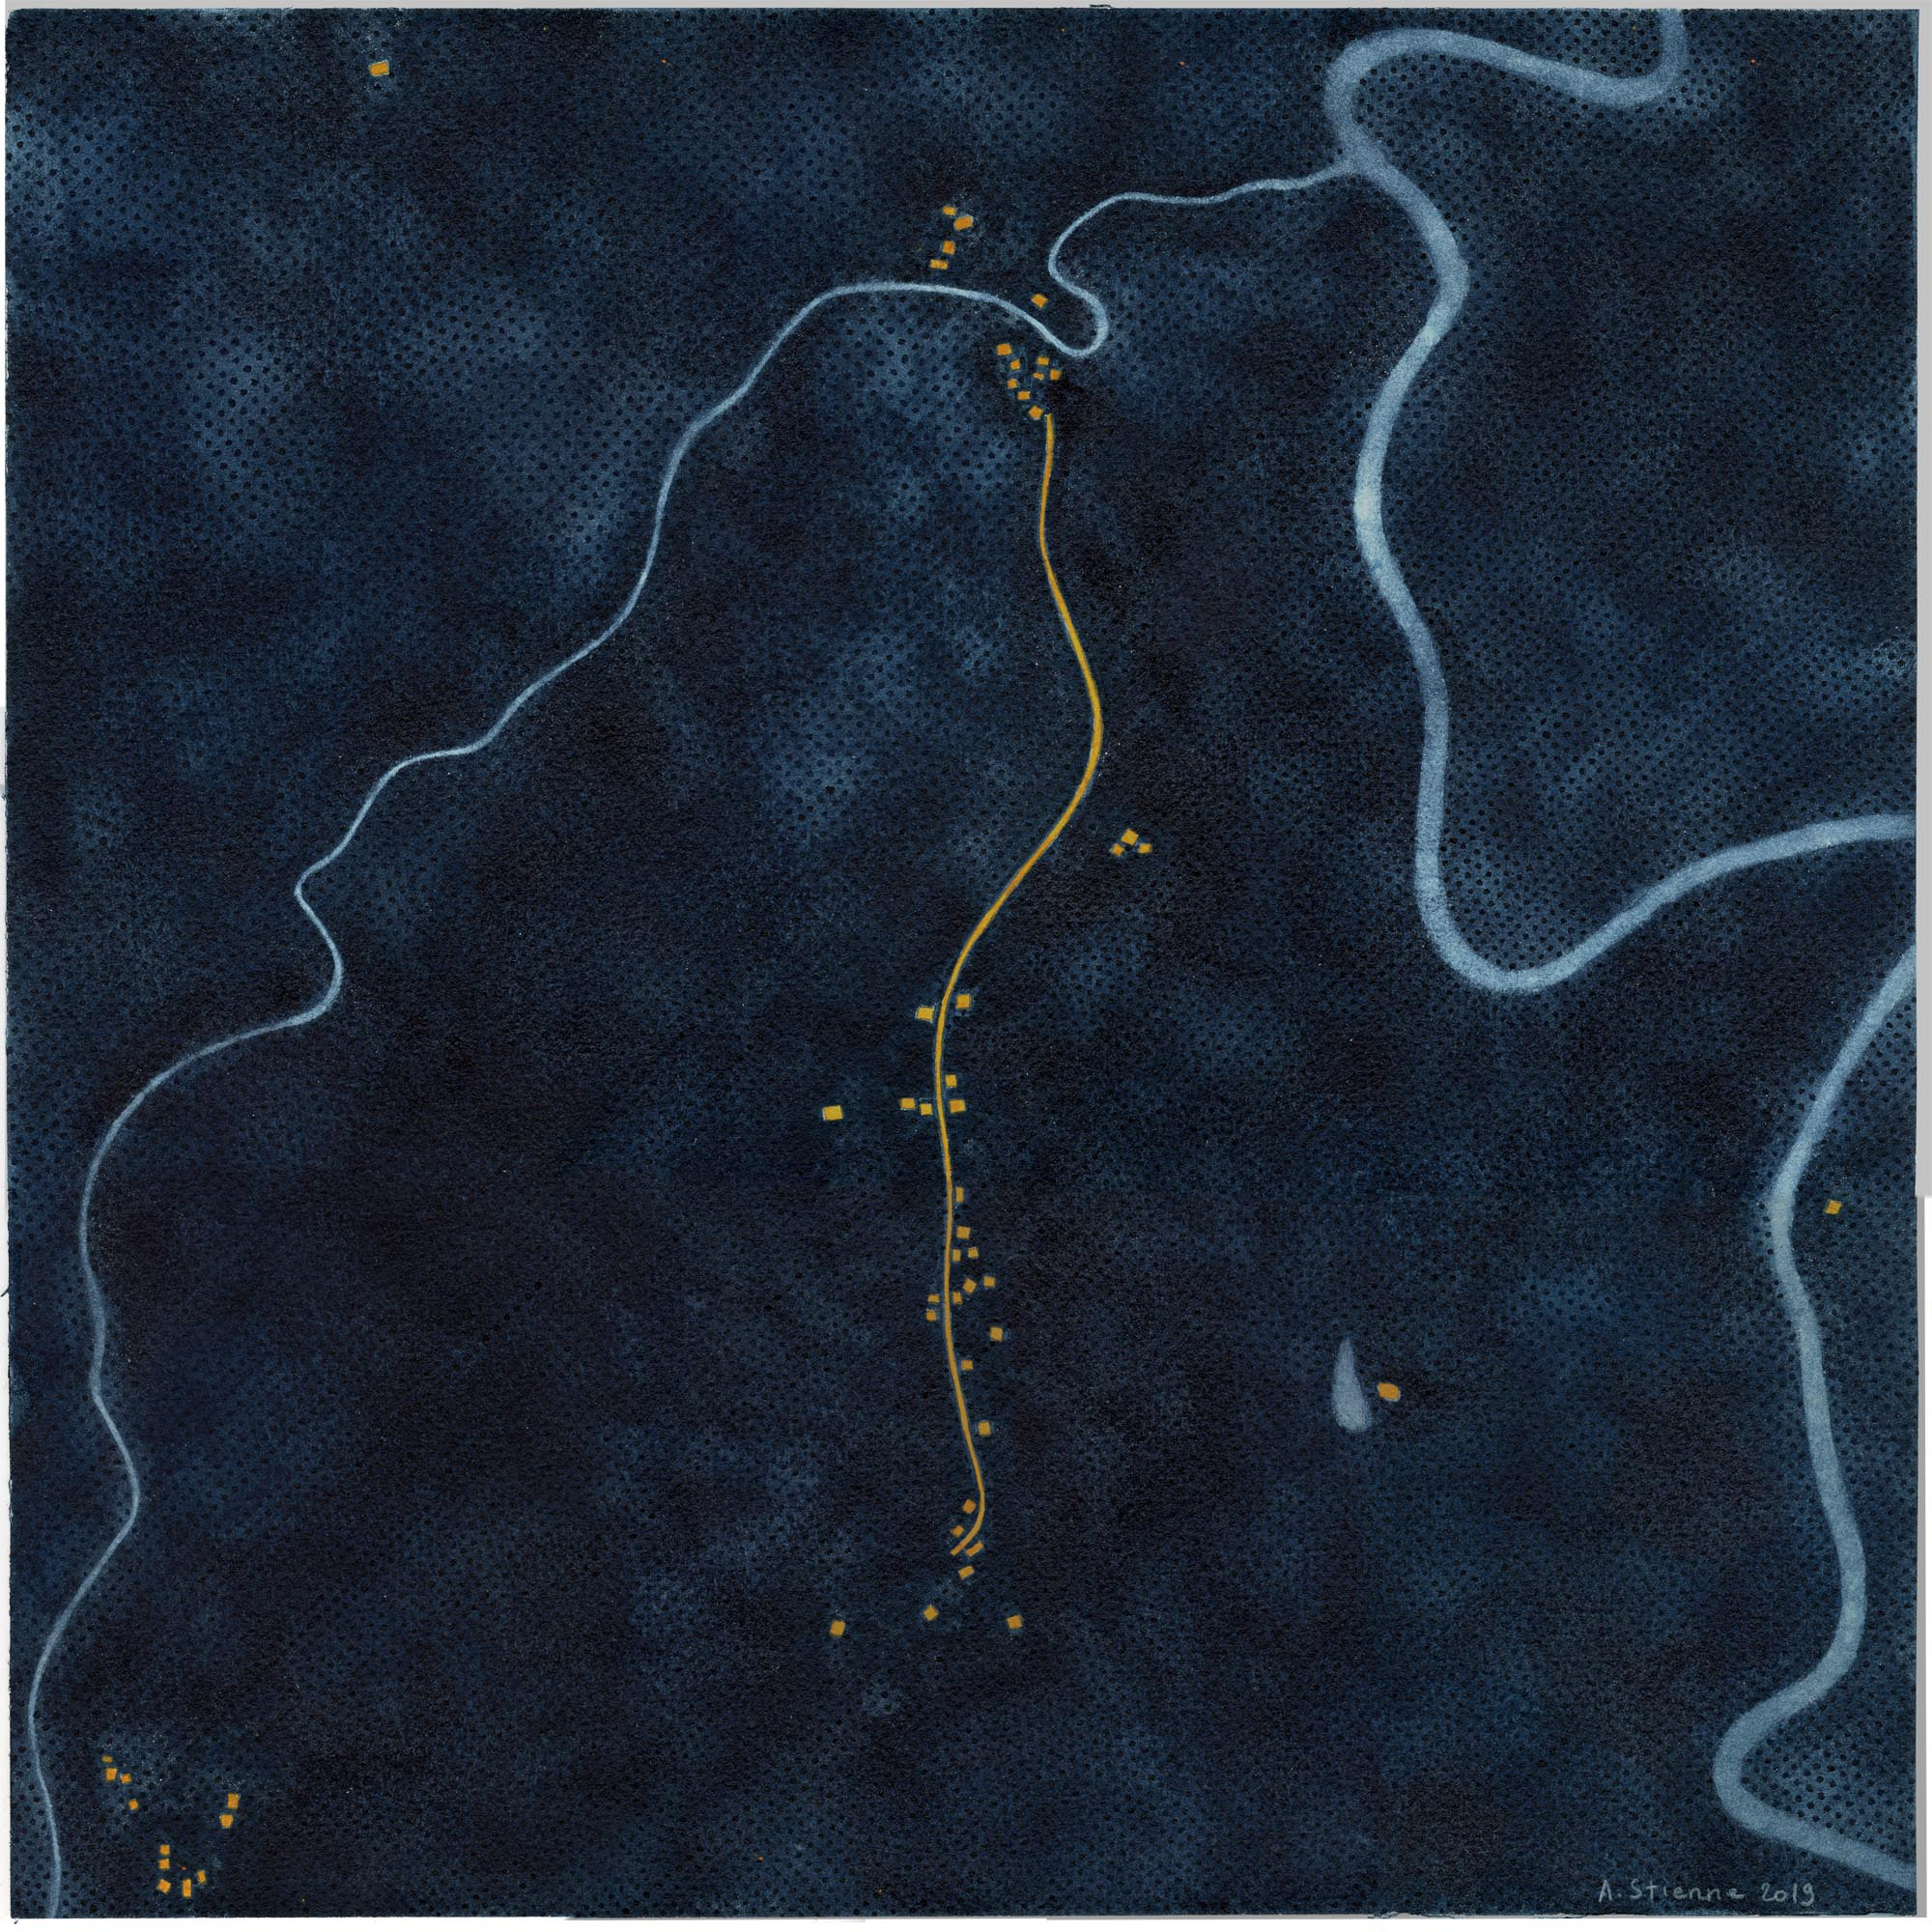
\includegraphics[height=4cm]{img/Honduras.jpg}

  \end{columns}
\end{frame}

\begin{frame}[c]{Doomed ?}
\vspace{-1cm}

\begin{figure}
  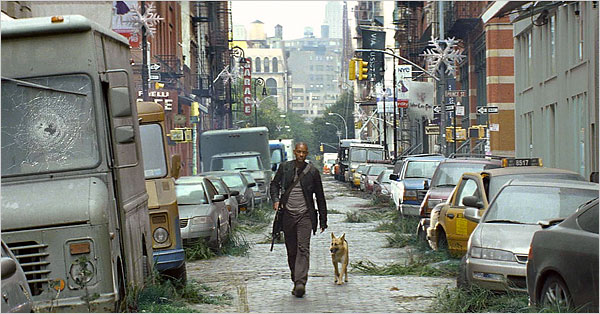
\includegraphics[width=\textwidth]{img/im_legend-600.jpg}
  \caption{I'm a legend (Francis Lawrence, 2007)}
\end{figure}
\end{frame}

\begin{frame}[c]{Approche par les Communs : un remede à l'effroi ?}
  \vspace{-1cm}
  \begin{columns}[onlytextwidth,T]
  \column{\dimexpr\linewidth-30mm-5mm}
    \begin{itemize}
      \item placer l'action collective au cœur de l'analyse (du diagnostic à la recherche de solution),
      \item faciliter et stimuler l'émergence d'arrangements institutionnels,
      \item remettre en cause l'externalisation des régulations.
    \end{itemize}
    Privilégier les fonctions et finalités des Communs plutôt que les structures
    \column{30mm}
    \vspace{2cm}
      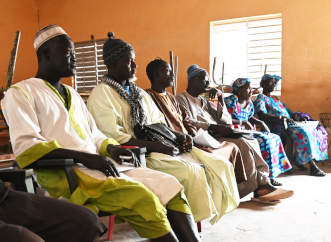
\includegraphics[height=3cm]{img/groupe_diohine.JPG}
  \end{columns}
\end{frame}

%-=-=-=-=-=-=-=-=-=-=-=-=-=-=-=-=-=-=-=-=-=-=-=-=
%	FRAME: Placer l'action collective au cœur
%-=-=-=-=-=-=-=-=-=-=-=-=-=-=-=-=-=-=-=-=-=-=-=-=

\section{Placer l'action collective au cœur}

\begin{frame}[c]{Le monde en Commun}
  \vspace{-1cm}
  \begin{columns}[onlytextwidth,T]
    \column{\dimexpr\linewidth-30mm-5mm}
      Une source d'inspiration chez H. Arendt (1957)
      \begin{itemize}
        \item On distingue le travail, l'oeuvre et l'action, 
        \item L'espace privé de l'espace public
        \item Le monde en commun est entre les Hommes. Il sépare autant qu'il rassemble
      \end{itemize}
  
    \small{
      \begin{alertblock}{\textsc{Deduction}}
        Les communs appartiennent au domaine public. Ils sont \textbf{négociés entre égaux}. Mais la réduction du domaine public réduit dans le même temps l’opportunité de faire du commun.
      \end{alertblock}
    }
  \column{30mm}
    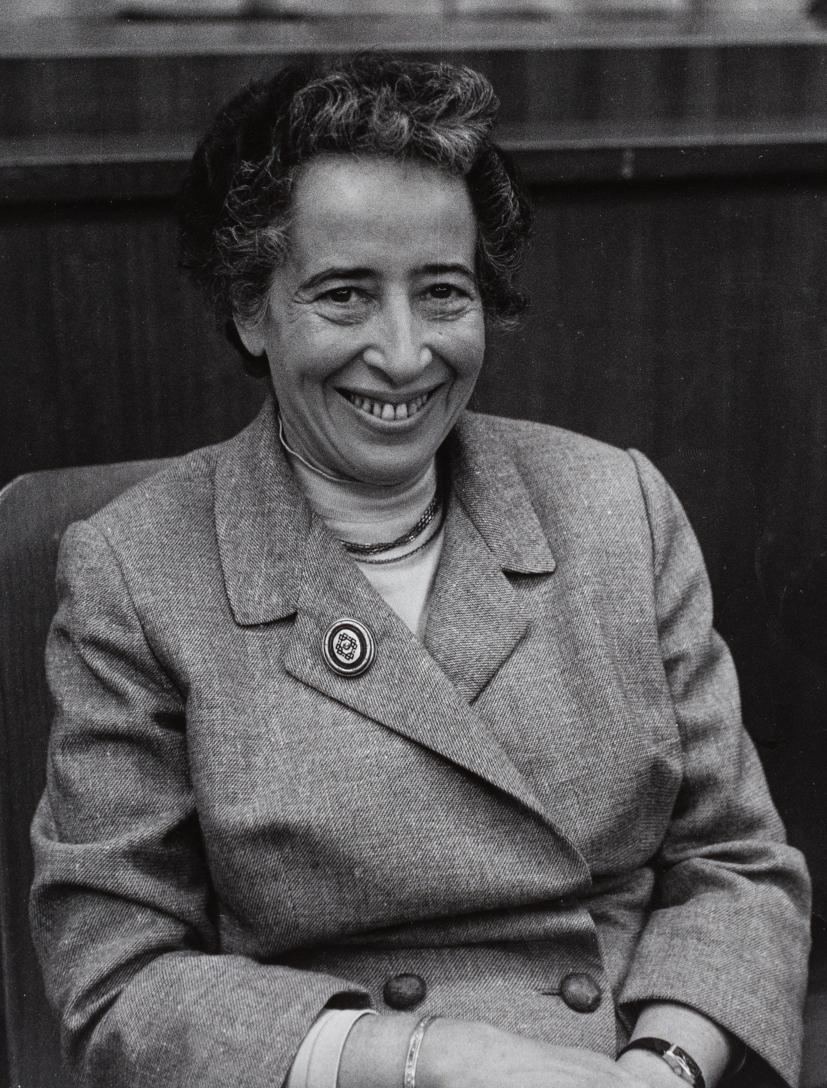
\includegraphics[height=5cm]{img/Hannah_Arendt.jpg}
    \end{columns}
  \end{frame}

  \begin{frame}[c]{Le décalage Prométhéen et l'urgence environnementale}
    \vspace{-1cm}
    \begin{columns}[onlytextwidth,T]
      \column{\dimexpr\linewidth-30mm-5mm}
      \begin{itemize}
        \item Dans \textit{"l'obsolessence de l'Homme"} Günther Anders (1956) propose la notionde décalage Prométhéen., 
        \item C'est les capacités de fabrication dépassant de très loin nos possibilités de représentation.
      \end{itemize}
      
      \small{
        \begin{alertblock}{\textsc{Une hypothese forte}}
          Accompagner les participants, c'est réduire le décalage Prométhéen, et permettre le passage a l'action.
        \end{alertblock}
      }
      \column{30mm}
      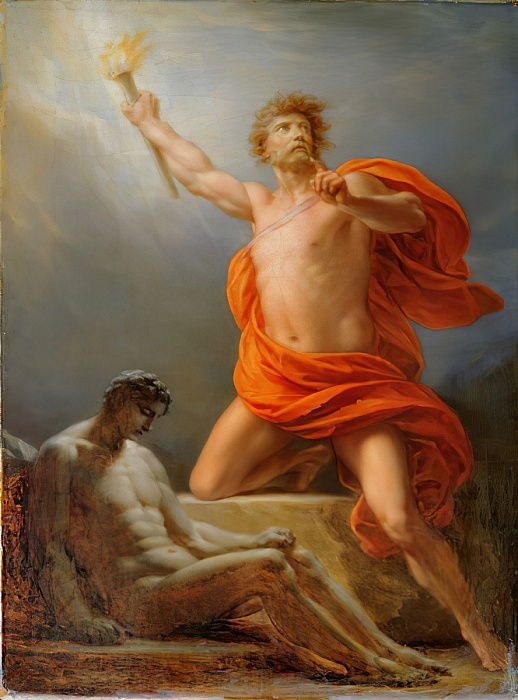
\includegraphics[height=5cm]{img/promethee.jpg}
    \end{columns}
  \end{frame}

  \begin{frame}[c]{Un exemple autour de la résolution du conflict a Diohine}
      \vspace{-1cm}
      \begin{columns}[onlytextwidth,T]
        \column{\dimexpr\linewidth-30mm-5mm}
        \begin{itemize}
          \item Droit Coutumier - Droit Moderne  
          \item Le chef de village à l'interface
          \item Une précéance de la coutume
        \end{itemize}
        
        \small{
          \begin{exampleblock}{\textsc{Illustration}}
            \begin{itemize}
              \item "Maintenant, vous comprennez mieux le fonctionnement du village que nos enfants."
              \item "Ici vous voyez on est bien moins libre que vous en ville"
              \item Il y a une obligation de moyen pour la paix sociale -- c'est un outils de production et d'action
            \end{itemize}
          \end{exampleblock}
        }
        \column{30mm}
        \vspace{1.5cm}
        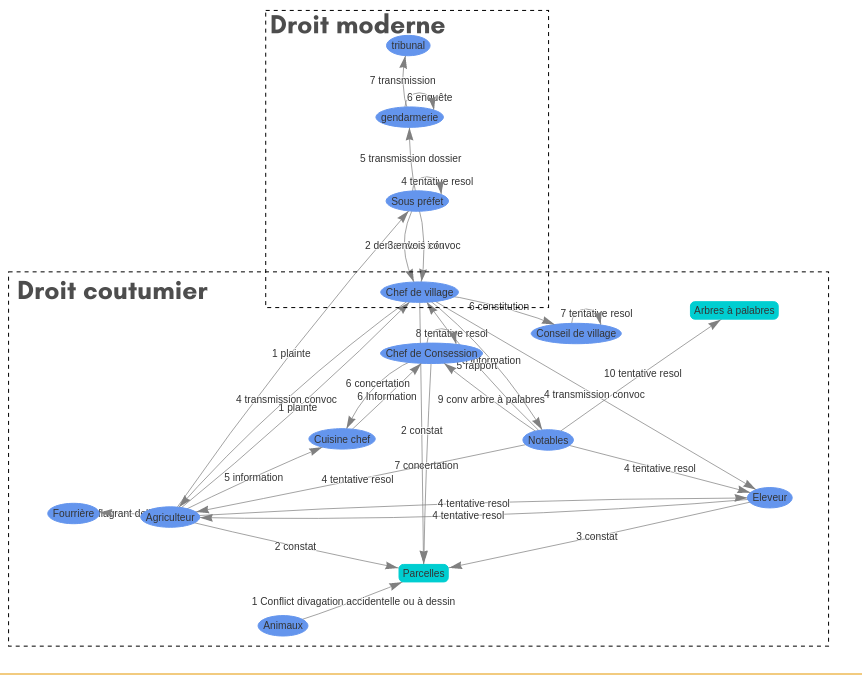
\includegraphics[height=5cm]{img/zone_droit_conflits.png}
      \end{columns}
    \end{frame}

%-=-=-=-=-=-=-=-=-=-=-=-=-=-=-=-=-=-=-=-=-=-=-=-=
%	FRAME: Faciliter et stimuler l'émergence d'arrangements
%-=-=-=-=-=-=-=-=-=-=-=-=-=-=-=-=-=-=-=-=-=-=-=-=

\section{Faciliter et stimuler l'emergence d'arrangements}

\begin{frame}[c]{L'égalité comme pré-requis}
  \vspace{-1cm}
  \begin{columns}[onlytextwidth,T]
    \column{\dimexpr\linewidth-30mm-5mm}
        \begin{itemize}
          \item Le \textit{"maître ignorant"} de Rancière (2003) qui accompagne : "contrairement à ce que laissent penser nos positions sociales, nous sommes égaux, voyons ce que nous pouvons en faire" 
          \item Le diplomate de Morizot (2020),  cherche les axes de mobilisation, car "une fois qu’on a circulé parmi les points de vue, on sent que certains n’ont pas la légitimité qu’ils réclament."
        \end{itemize}
  
        \small{
            \begin{alertblock}{\textsc{Une posture philosophique}}
              Entre Rancière et Morizot, on a les composante de la posture des acteurs du vivre ensemble.
            \end{alertblock}
          }
    \column{30mm}
    \vspace{0.5cm}
          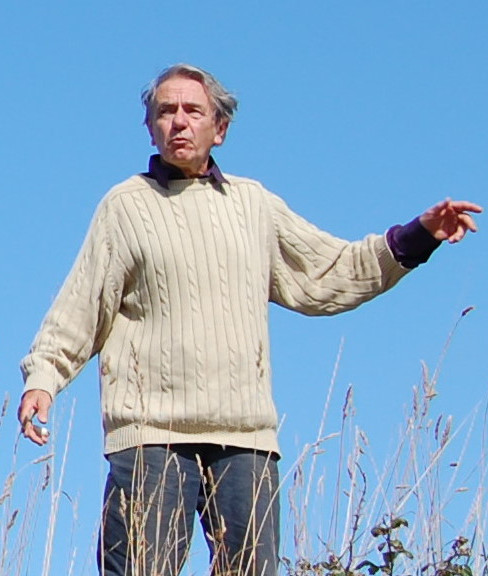
\includegraphics[width=3cm]{img/Ranciere.jpg}\\
          
\includegraphics[width=3cm]{img/morizot.jpg}
  \end{columns}
\end{frame}

\begin{frame}[c]{Où intervenir ?}
    \vspace{-1cm}

   La grille de lecture TORSO (TerritOry-Resources Societal Organization) (Maraud et Delay, 2022) donner a voirs les difficultées d'égalité? 
  \begin{center}
   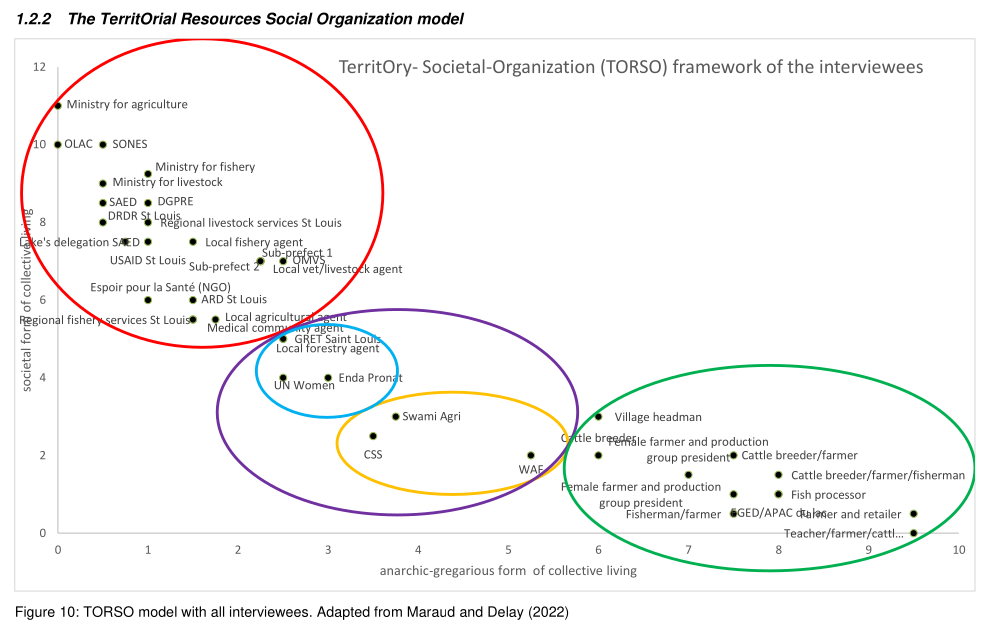
\includegraphics[width=9cm]{img/torso_mathilde.png}
  \end{center}

\end{frame}

\begin{frame}[c]{Formaliser les arrangements : \textit{institutional Grammar 2.0}}
    \vspace{-1cm}
    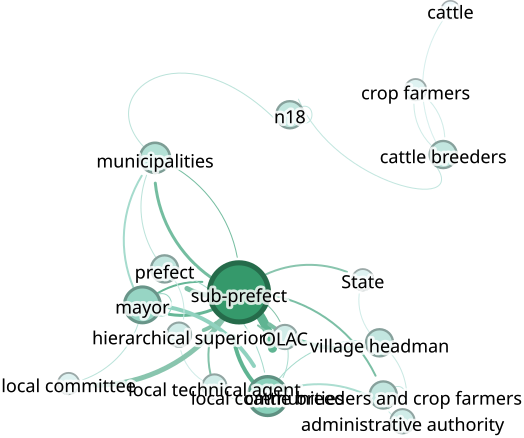
\includegraphics[height=4cm]{img/sg_agent_Admin.png}
    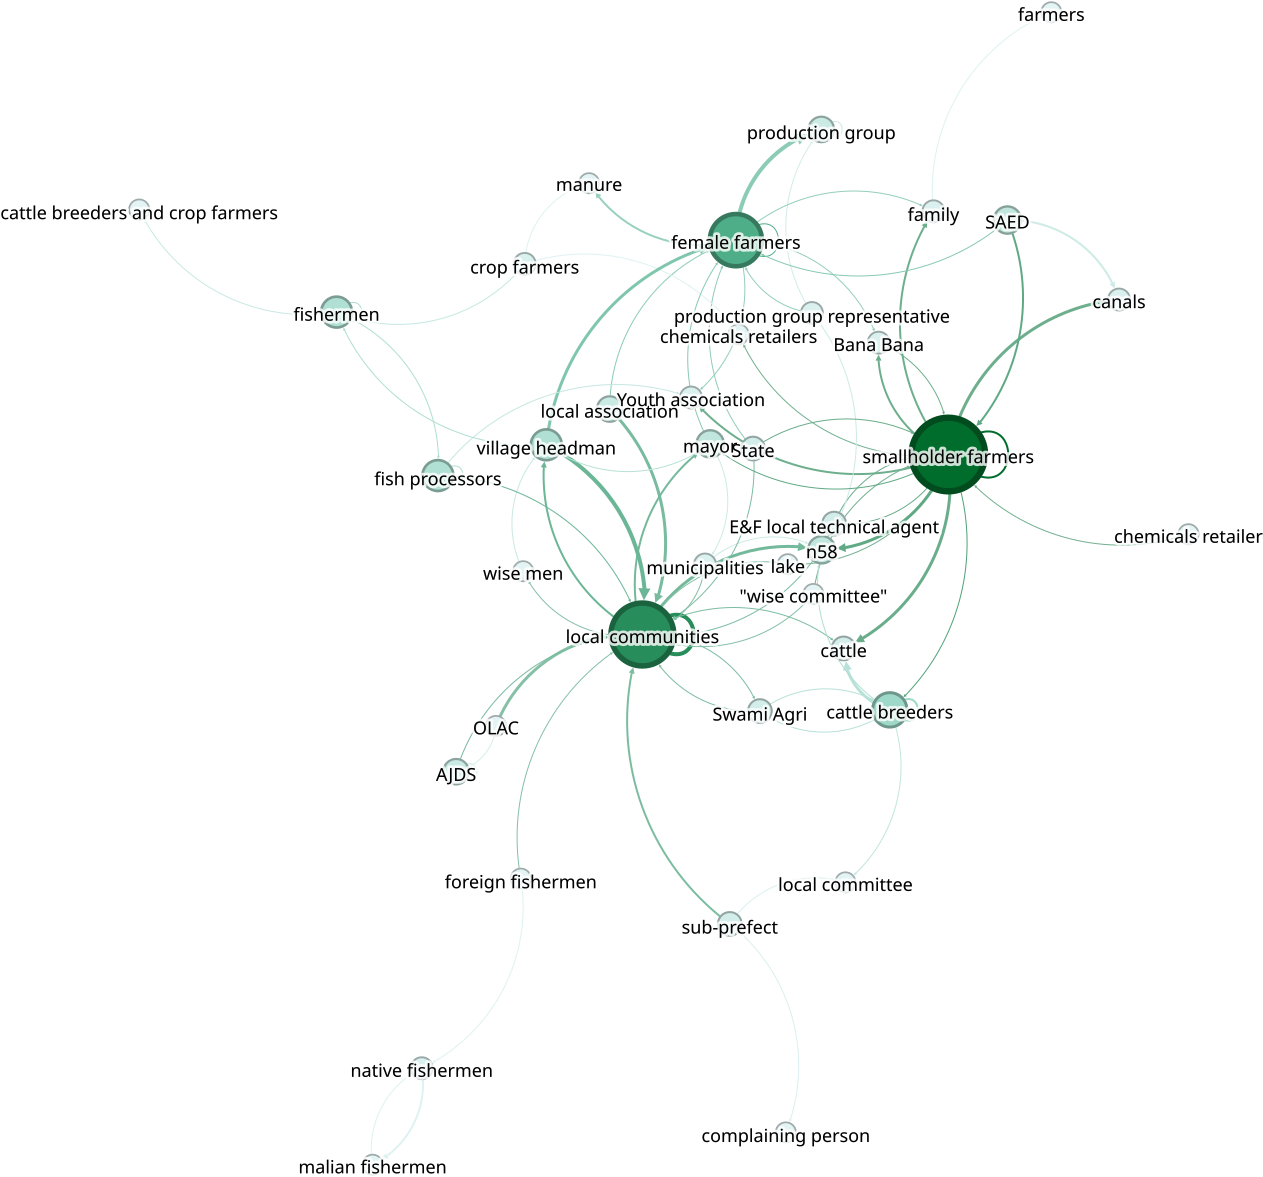
\includegraphics[height=5cm]{img/sg_popLozc.png}
\end{frame}

  \begin{frame}[c]{La maturité des Communs}
    \vspace{-1cm}
    
    \small{
      \begin{alertblock}{\textsc{Une hypothese forte}}
        la société produit de l’égalité. Cette égalité produit (mécaniquement) une forme de nivellement (conformisme). En s’attaquant a la société par le prisme de l’intime Rousseau et les Romantique faisait l’éloge de la pluralité qui est la nécessité d'une société en bonne santé. Dans une société, il faut donc arriver à maintenir la chose dans un équilibre précaire entre égalité et pluralité. Ce qui doit nécessairement induire une dépense d’énergie. (pour ne pas faire augmenter l'entropie). 
      \end{alertblock}
    }
  
  \end{frame}
  
  \begin{frame}[c]{La maturité des communs}
      \vspace{-1cm}
      
    Un travail conjoint avec Le GRET qui conçoit trois catégories de communs différents :
      \begin{itemize}
          \item la ressource en tant que commun (nommé aussi “commun de ressource”),
          \item le service en tant que commun (ou “commun de service”)
          \item le territoire en tant que commun.
      \end{itemize}
      
       \small{
         \begin{alertblock}{\textsc{Vers le territoire et au-dela}}
           On entre toujours par une ressource, autour de laquelle les utilisateurs se structurent pour petit à petit structurer un service (une émergence) et, quand plusieurs réseaux de communs se croisent sur un même territoire, on commence à identifier ce territoire comme un commun.
         \end{alertblock}
       }
  \end{frame}
      
  \begin{frame}[c]{Le GRET acteur du vivre ensemble dans les Niayes}
      \vspace{-1cm}
      \begin{columns}[onlytextwidth,T]
        \column{\dimexpr\linewidth-30mm-5mm}
        \begin{itemize}
            \item le GRET se situe d’un point de vue “politique” (au sens de H. Arendt 1958 (re-éd. 2020) ou de C. Mouffe, 2018). Il prend en charge le maintien des relation,
            \item Cette progression vers un territoire en tant que commun va de pair avec une mise à jour dans l’espace public de ces réseaux de solidarité.
        \end{itemize}
        \column{30mm}
        \vspace{0.5cm}
         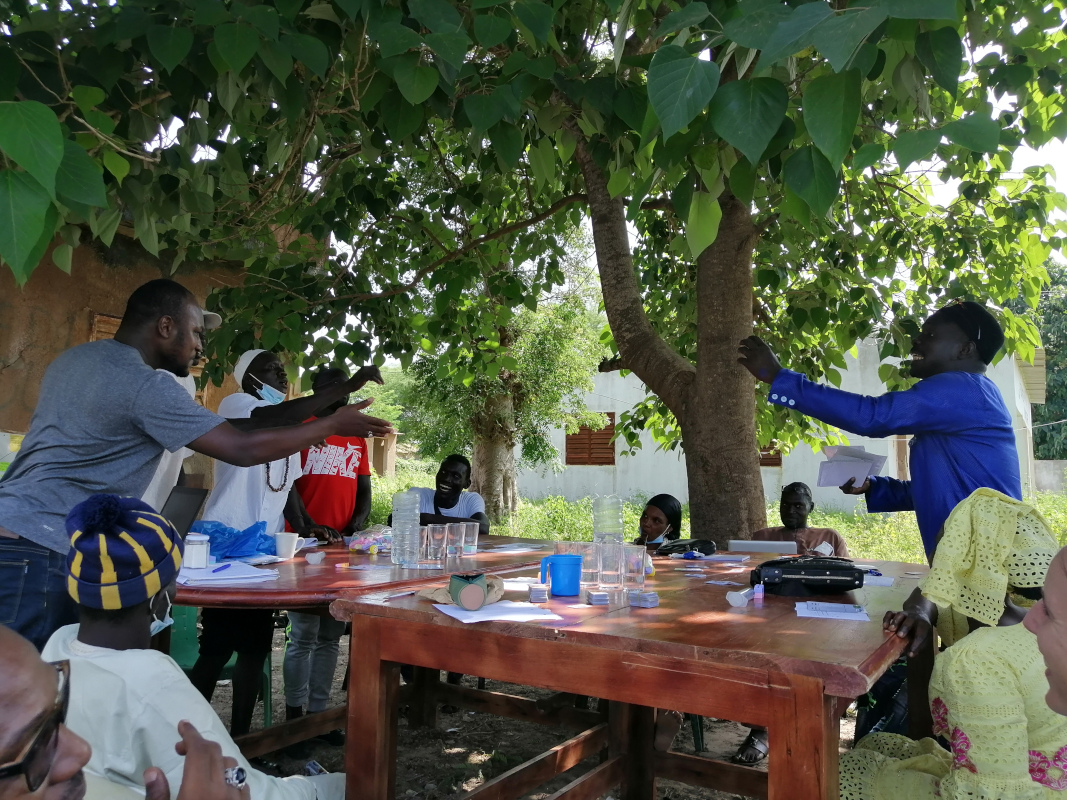
\includegraphics[height=3cm]{img/atelier_montroland.jpg}
      \end{columns}
  \end{frame}
      
      
  \begin{frame}[c]{Des formes de gouvernance : GIREL}
      \vspace{-1cm}
      \begin{itemize}
          \item Une entrée par la ressource eau, et des acteurs homogènes, puis une recherche de pluralité.
          \item plusieurs usages peuvent être concurrents : l’usage des maraîchers VS éleveurs $\rightarrow$ service en temps que commun $\rightarrow$ De nouveaux attributs (suivi-évaluation)
      \end{itemize}
      \begin{figure}
          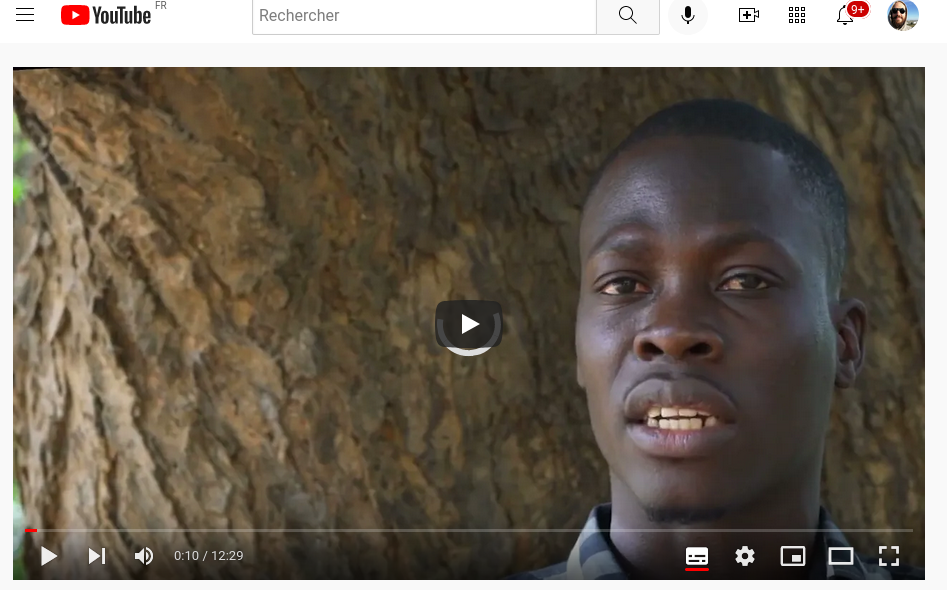
\includegraphics[height=3.5cm]{img/ComMod_f'eauDiem.png}
          
\includegraphics[height=3.5cm]{img/qrcode_feaudiem.png}
      \end{figure}
      
      \end{frame}
      
      \begin{frame}[c]{Des formes de gouvernance : GPSE}
      \vspace{-1cm}
      \begin{itemize}
          \item La prise en compte de la pluralité des acteurs permet la coexistence de l’égalité (entre eux) et de la distinction (considérer chacun comme unique).
          \item La Paix sociale, un système de valeur puissant au Sénégal!
          \item Un \textbf{acteur du vivre ensemble} qui cherche a maintenir la relation entre usager et ressources, quelque soit le système autour (qualité de service)
      \end{itemize}
       \small{
         \begin{alertblock}{\textsc{Qu'est-ce qui propulse le systeme : les valeurs }}
          Si le système a été envisagé avec des composants “législateurs” externes au système, le contrat de confiance entre eux et les acteurs/composants du système implique un consentement préalable (ou des mesures de coercition).
         \end{alertblock}
       }
      \end{frame}

%-=-=-=-=-=-=-=-=-=-=-=-=-=-=-=-=-=-=-=-=-=-=-=-=
%	FRAME: Remettre en cause l'externalisation des régulations
%-=-=-=-=-=-=-=-=-=-=-=-=-=-=-=-=-=-=-=-=-=-=-=-=

\section{Remettre en cause l'externalisation des regulations}

\begin{frame}[c]{La viabilité}
  \vspace{-1cm}
  \begin{itemize}
    \item La viabilité de A. Tsing (\textit{liviability}) ; "la question « est-ce viable ? » serait peut-être la question rationnelle par excellence, une question qui implique l'ensemble de ce, humain et non-humain, qui vivent les uns grâce aux autres, par les autres, au risque des autres."
    \item la viabilité de Aubin et Saint Pierre ; La théorie de la viabilité s’intéresse au noyau de viabilité, qui recouvre l’ensemble des états permettant à un modèle ou à un système d’être viable et de le rester dans le temps. Un noyau de viabilité dépend de la position des contraintes que l’on fait peser sur le système.
  \end{itemize}


\end{frame}

\begin{frame}[c]{Diohine : viabilité au sens de Tsing}
    \vspace{-1cm}
    \begin{itemize}
      \item La viabilité de A. Tsing (\textit{liviability})
      \item la viabilité de Aubin et Saint Martin
    \end{itemize}
  
  
\end{frame}

\begin{frame}[c]{Lac de Guiers : viabilité au sens  d'Aubin}
      \vspace{-1cm}
      \begin{itemize}
        \item La viabilité de A. Tsing (\textit{liviability})
        \item la viabilité de Aubin et Saint Martin
      \end{itemize}
    
    
\end{frame}

\begin{frame}[c]{Commun et viabilité}
  \vspace{-1cm}
  \begin{itemize}
    \item La viabilité de A. Tsing (\textit{liviability})
    \item la viabilité de Aubin et Saint Martin
  \end{itemize}


\end{frame}

%-=-=-=-=-=-=-=-=-=-=-=-=-=-=-=-=-=-=-=-=-=-=-=-=
%	FRAME: OLDY
%-=-=-=-=-=-=-=-=-=-=-=-=-=-=-=-=-=-=-=-=-=-=-=-=

\section{Un genre de conclusion ?}

\begin{frame}[c]{}
\vspace{-1cm}
\begin{itemize}
    \item Les rapports de force sont facilités quand le système ignore certaines parties de lui-même (absence d'émergence forte).
    \item La paix sociale a ouvert la voie sur les temporalités du droit (circulaire/éternelle - linéaire/immortelle )
    \item "nul n'est passif dans ces histoires mais toute activité y est précaire, ne persiste que sous le signe d'une interdépendance" (Stengler 2017)
\end{itemize}

\begin{figure}
  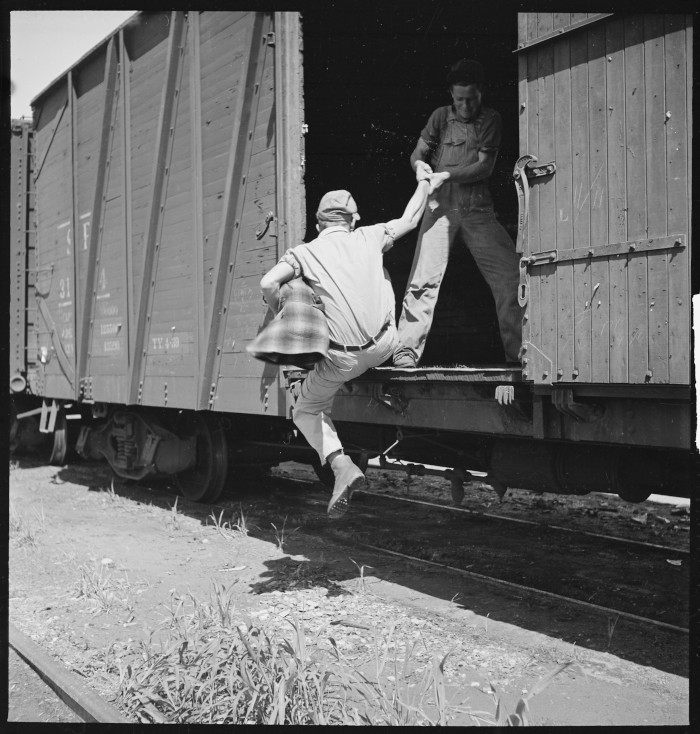
\includegraphics[height=4cm]{img/valeurs.jpg}
\end{figure}


\end{frame}

%-=-=-=-=-=-=-=-=-=-=-=-=-=-=-=-=-=-=-=-=-=-=-=-=
%	FRAME: MERCI DE VOTRE ATTENTION
%-=-=-=-=-=-=-=-=-=-=-=-=-=-=-=-=-=-=-=-=-=-=-=-=
{
\usebackgroundtemplate{
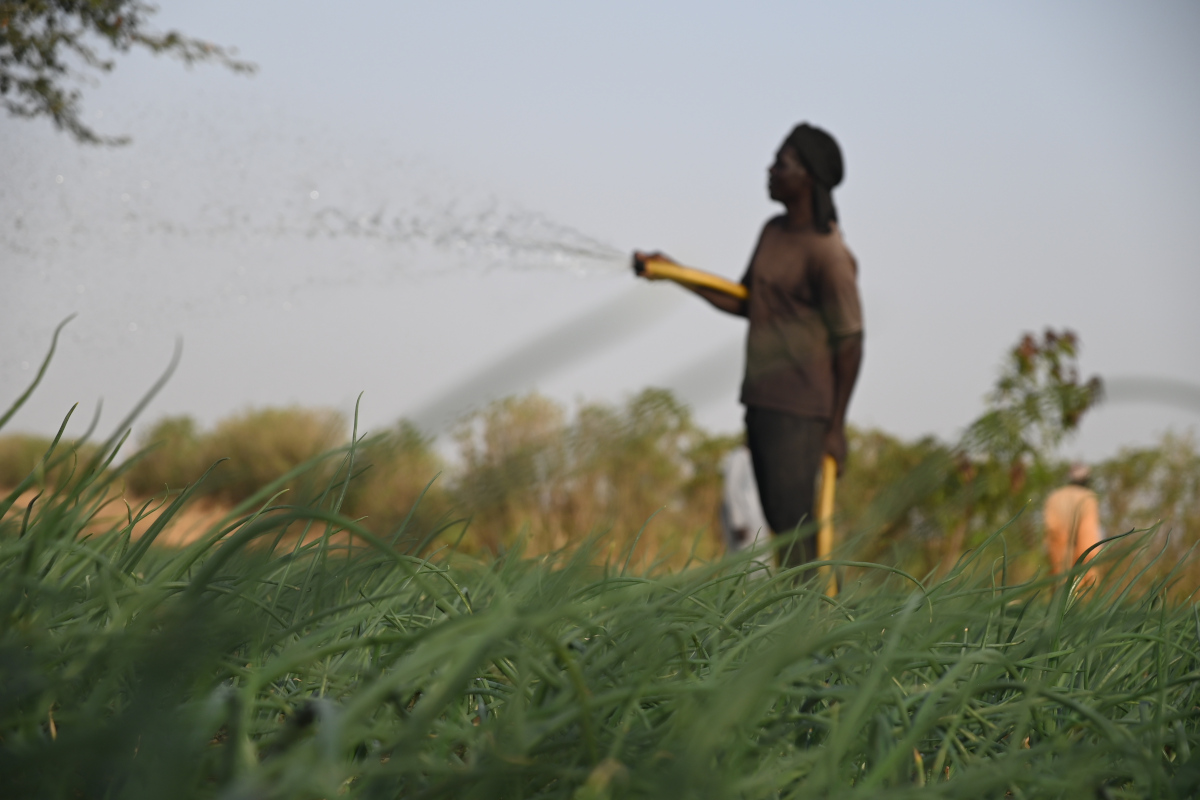
\includegraphics[width=\paperwidth]{img/arroseur_diohine.JPG}}%
\begin{frame}
  \vspace{-1em}
  \begin{minipage}[t][.8\textheight]{\textwidth}
    \color{\cnGrey}{\LARGE{Merci de votre attention}}

    \vfill

  %\hfill \small{Photo credit : Thomas m-louis. sur \includegraphics[height=0.55cm]{img/flickr_logo}}
  \end{minipage}
  \vspace{-3.5em}
  \centering
	You can find this presentation on github
\includegraphics[height=0.85cm]{img/github}

\end{frame}
}


\end{document}
